\documentclass[aspectratio=169,xcolor=dvipsnames]{beamer}
\usetheme{SimpleDarkBlue}

\usepackage{hyperref}
\usepackage{graphicx}
\usepackage{booktabs}
\usepackage{amsmath,amssymb,mathtools}
\usepackage{fontspec}
\usepackage{luatexja}
\usepackage{appendixnumberbeamer}

\setmainfont{Alegreya Sans Light}[
  ItalicFont={* Italic},
  BoldFont={Alegreya Sans Medium},
  BoldItalicFont={Alegreya Sans Medium Italic}]
\setsansfont{Alegreya Sans Light}[
  ItalicFont={* Italic},
  BoldFont={Alegreya Sans Medium},
  BoldItalicFont={Alegreya Sans Medium Italic}]

\AtBeginSection[]{
  \begin{frame}[noframenumbering, plain]
    \Huge{\centerline{\textbf{\insertsection}}}
  \end{frame}
}

\let\tempone\itemize
\let\temptwo\enditemize
\renewenvironment{itemize}{\tempone\addtolength{\itemsep}{\fill}}{\temptwo}
\let\tempa\enumerate
\let\tempb\endenumerate
\renewenvironment{enumerate}{\tempa\addtolength{\itemsep}{\fill}}{\tempb}

\defbeamertemplate*{footline}{shadow theme}{%
    \leavevmode\hbox{%
        \hypersetup{linkcolor=white,urlcolor=white,citecolor=white}
        \begin{beamercolorbox}[wd=1.02\paperwidth, ht=2.5ex, dp=1.125ex, leftskip=.3cm plus1fil, rightskip=0.3cm]{author in head/foot}%
            \insertsectionnavigationhorizontal{.80\textwidth}{}{} \hspace{.3cm} \hfill \#\ \insertframenumber \ / \ \inserttotalframenumber%
        \end{beamercolorbox}%
    }%
}
\setbeamertemplate{footline}[shadow theme]
\setbeamertemplate{navigation symbols}{}

\providecommand{\blue}[1]{\textcolor{RoyalBlue}{#1}}
\providecommand{\red}[1]{\textcolor{BrickRed}{#1}}

\title[Endogenous Growth]{Endogenous Growth}
\author[Hui-Jun Chen]{Hui-Jun Chen}
\institute[]{National Tsing Hua University\\Department of Economics}
\date{Based on Julia K. Thomas, Topic 4}

\begin{document}

\begin{frame}[plain,noframenumbering]
    \titlepage
\end{frame}

\section{Motivation}

\begin{frame}{Kaldor facts: what should a long-run growth model explain?}
\small
Economic data over long periods (especially for the U.S. and U.K.) suggest:
\begin{enumerate}
    \item roughly constant \blue{capital and labor shares} of national income,
    \item roughly constant \blue{growth rate of the capital stock},
    \item roughly constant \blue{growth rate of output per worker},
    \item roughly constant \blue{capital--output ratio},
    \item roughly constant \blue{rate of return on investment}, and
    \item steadily \blue{growing real wages}.
\end{enumerate}

\vspace{0.4em}
\textbf{Implication.} A useful growth model should deliver a \blue{balanced growth path}: 
\begin{itemize}
    \item factor shares are stable,
    \item aggregate quantities grow at regular rates,
    \item the return to capital is stable, and
    \item wages rise with productivity.
\end{itemize}
\end{frame}

\begin{frame}{Kaldor facts in a neoclassical growth model}
\small
Kaldor's observations lead us to emphasize balanced growth paths with:
\begin{itemize}
    \item \blue{constant factor shares},
    \item \blue{capital and output growing at a common rate},
    \item \blue{output per worker and capital per worker moving together},
    \item a \blue{constant rental rate on capital}, and
    \item \blue{growing real wages}.
\end{itemize}

\vspace{0.4em}
These observations guide common functional-form choices:
\begin{enumerate}
    \item \textbf{Cobb--Douglas production}: helps deliver stable factor shares.
    \item \textbf{Separable CES preferences}: helps support balanced growth with stable labor supply behavior.
    \item Together with common growth in $Y$ and $K$, these help generate growing real wages.
\end{enumerate}
\end{frame}

\begin{frame}{Exact figure from the source: capital-to-GDP roughly constant despite growth}
\centering
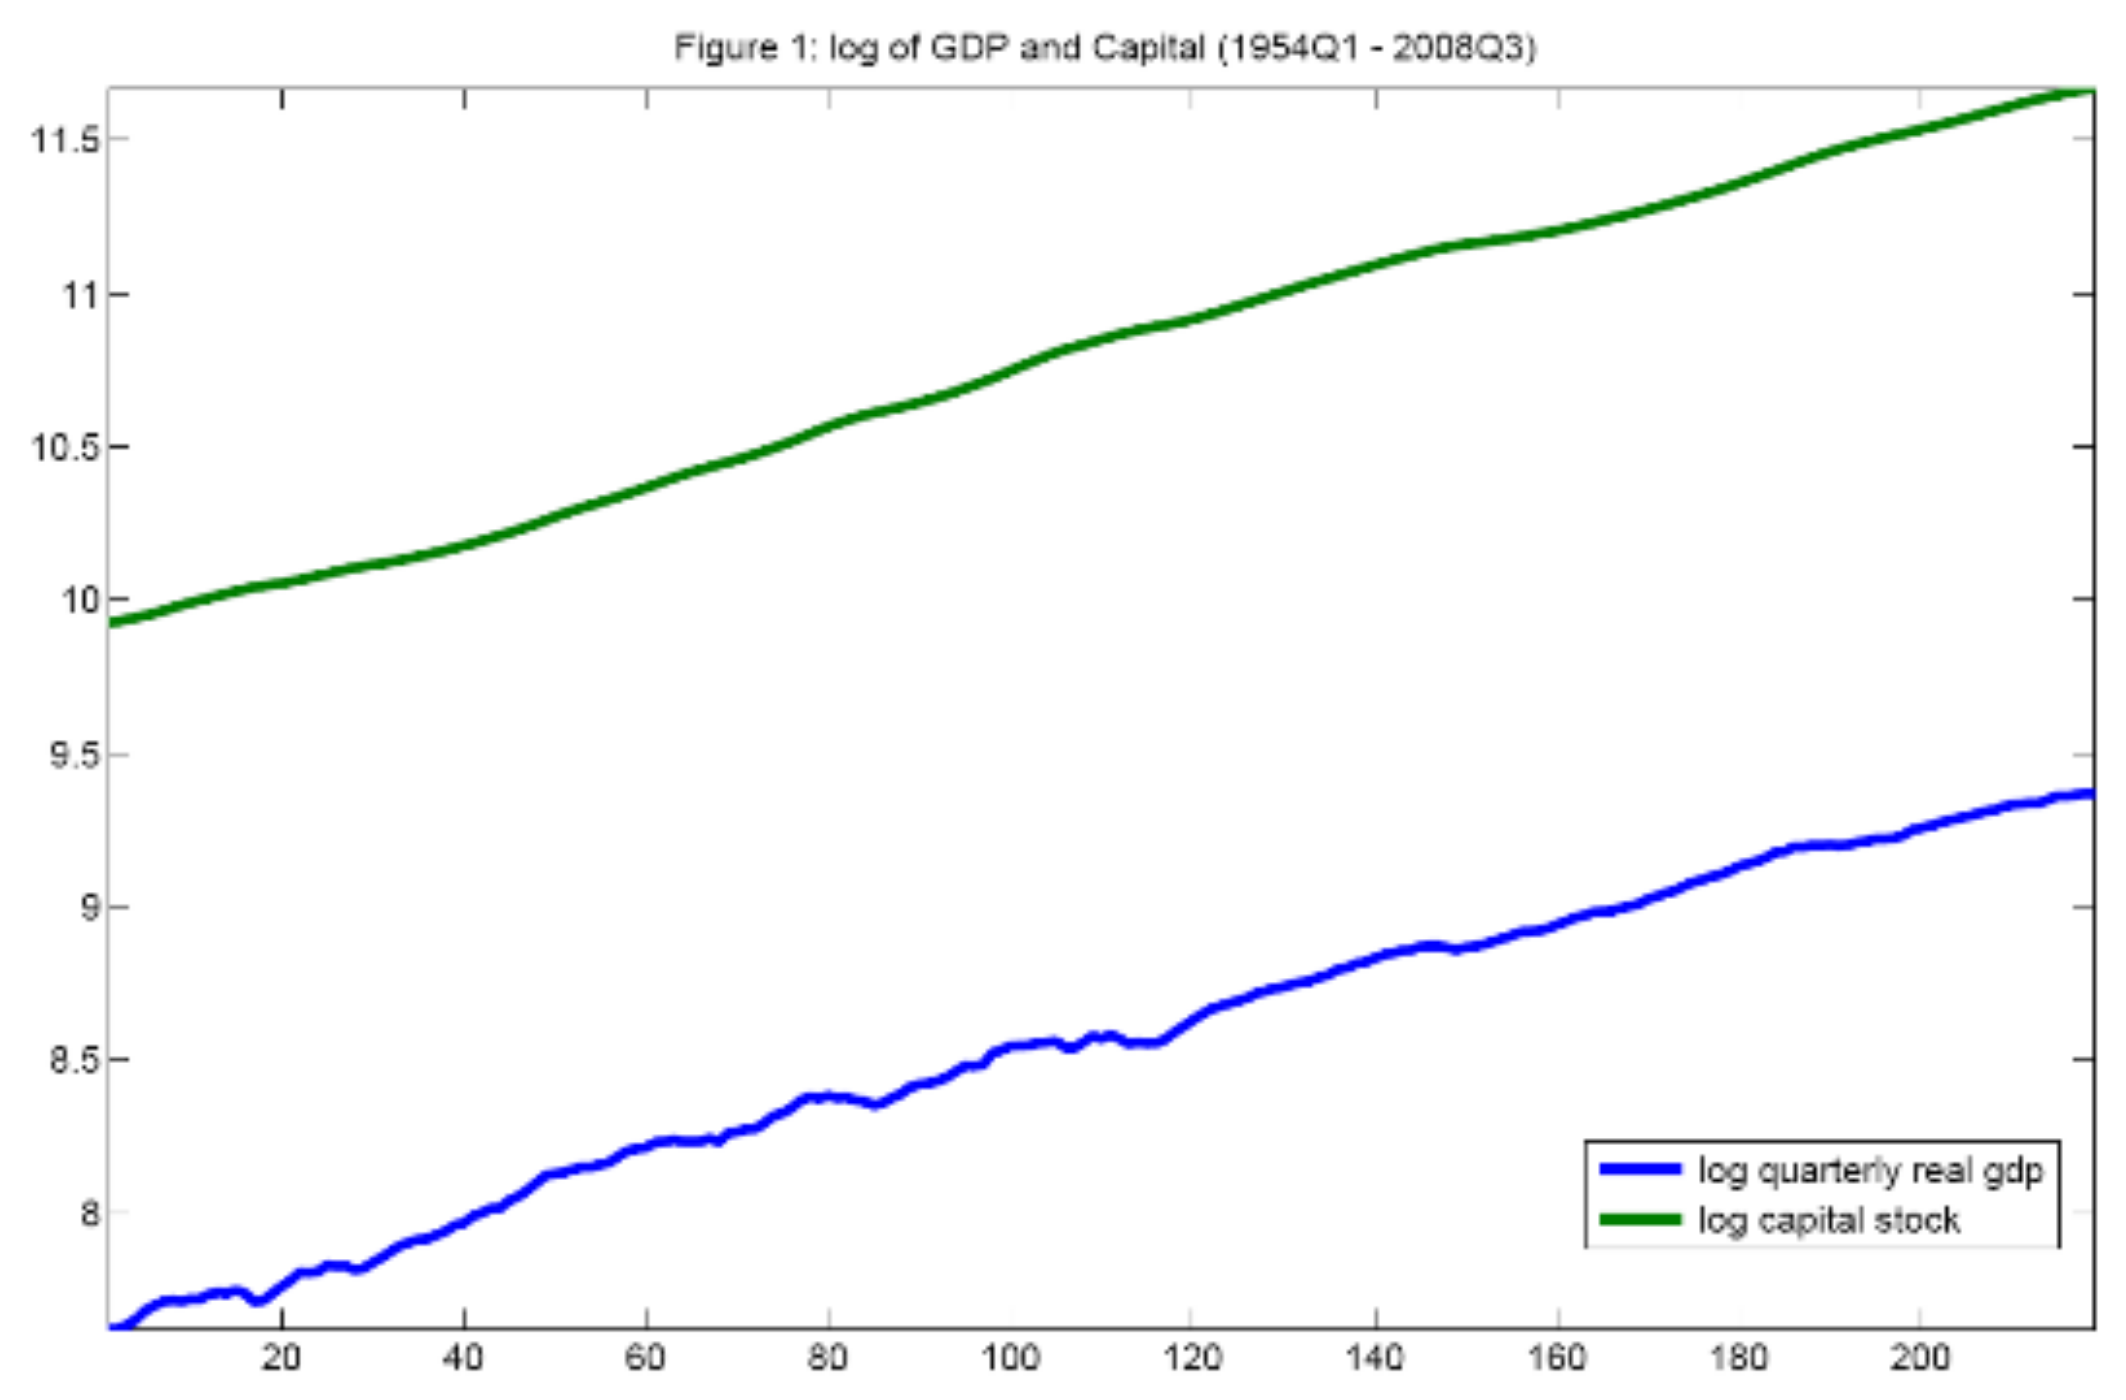
\includegraphics[width=0.95\textwidth]{topic4_p04_figure.png}
\end{frame}

\begin{frame}{Exact figure from the source: dispersion in per-capita income levels}
\centering
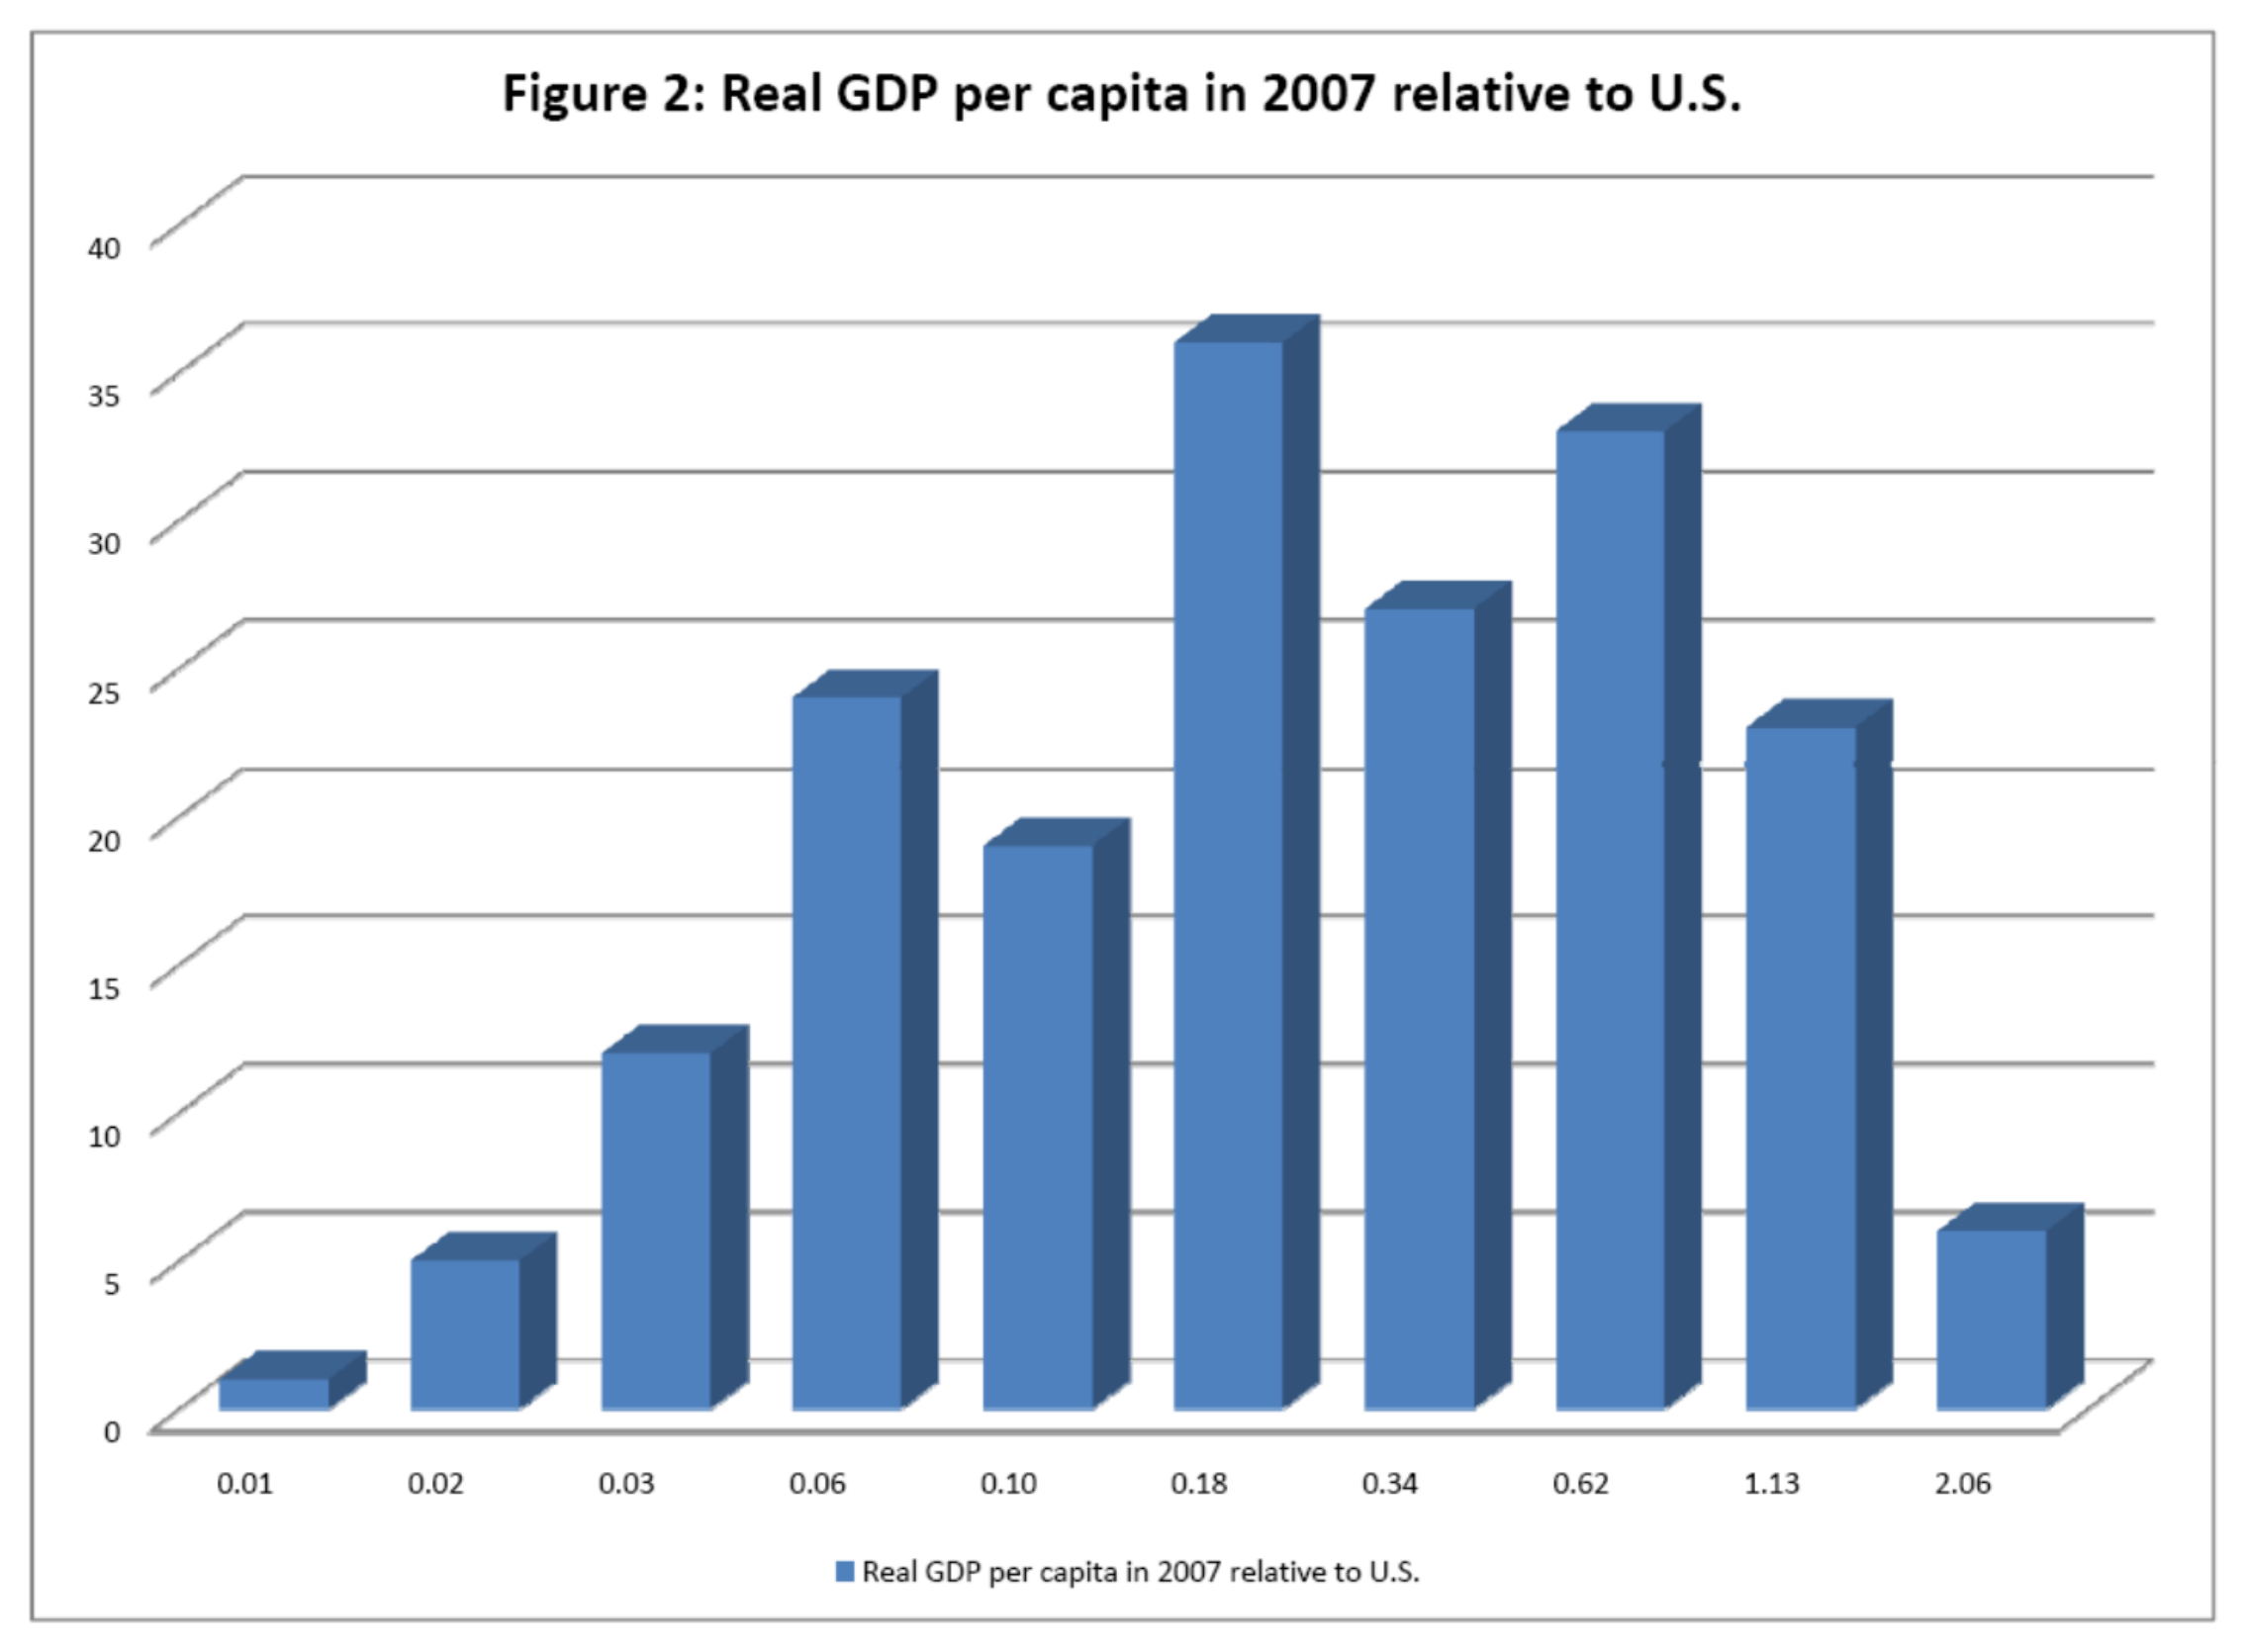
\includegraphics[width=0.88\textwidth]{topic4_p05_figure.png}
\end{frame}

\begin{frame}{Exact figure from the source: dispersion in per-capita growth rates}
\centering
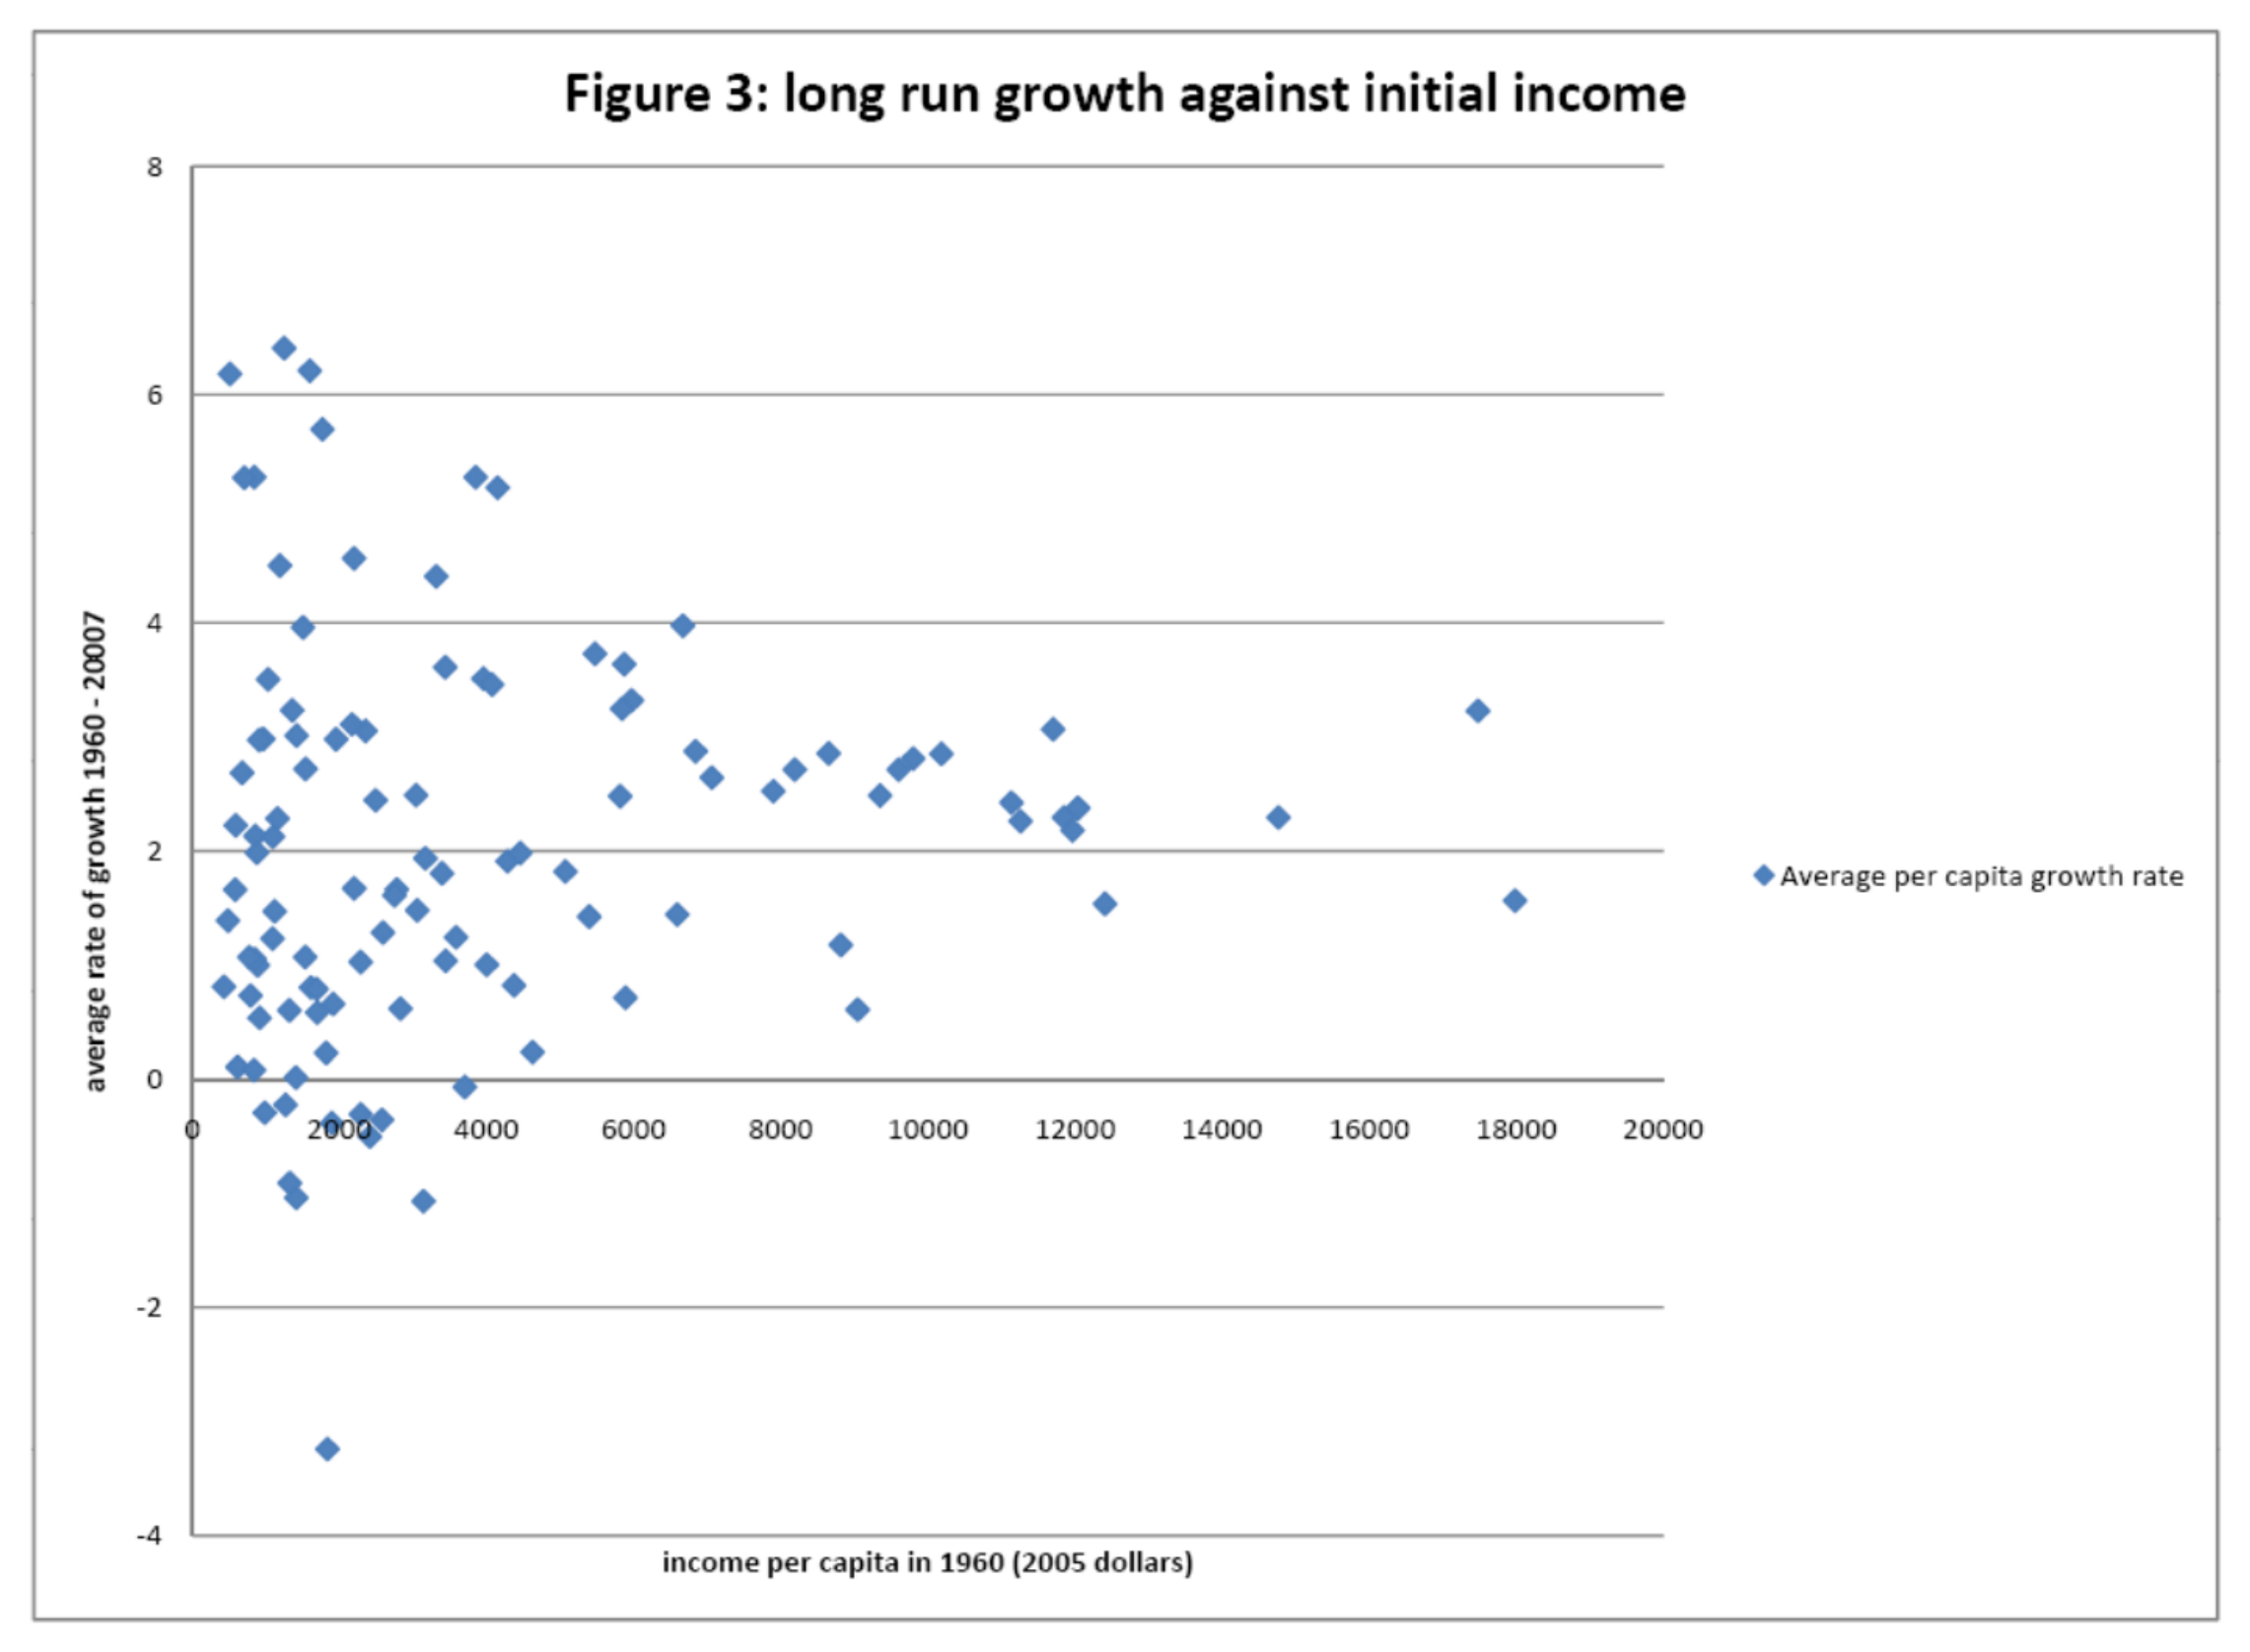
\includegraphics[width=0.88\textwidth]{topic4_p06_figure.png}
\end{frame}

\begin{frame}{Development accounting: where do income differences come from?}
\small
Suppose production is CRS in physical capital and efficiency units of labor:
\[
Y = K^{\alpha}(AhL)^{1-\alpha}.
\]
Then output per person can be decomposed as
\[
\frac{Y}{\mathrm{pop}} =
\left(\frac{K}{Y}\right)^{\frac{\alpha}{1-\alpha}}
\left(\frac{L}{\mathrm{pop}}\right) h A.
\]

\begin{itemize}
    \item $\frac{K}{Y}$ captures \blue{capital intensity}.
    \item $\frac{L}{\mathrm{pop}}$ captures \blue{labor-force participation / hours}.
    \item $h$ captures \blue{human capital}.
    \item $A$ captures \blue{total factor productivity (TFP)}.
\end{itemize}

\vspace{0.4em}
A key empirical lesson from development accounting is that \blue{TFP differences explain a large share of cross-country income gaps}.
\end{frame}

\begin{frame}{Exact figure from the source: TFP's role in cross-country income differences}
\centering
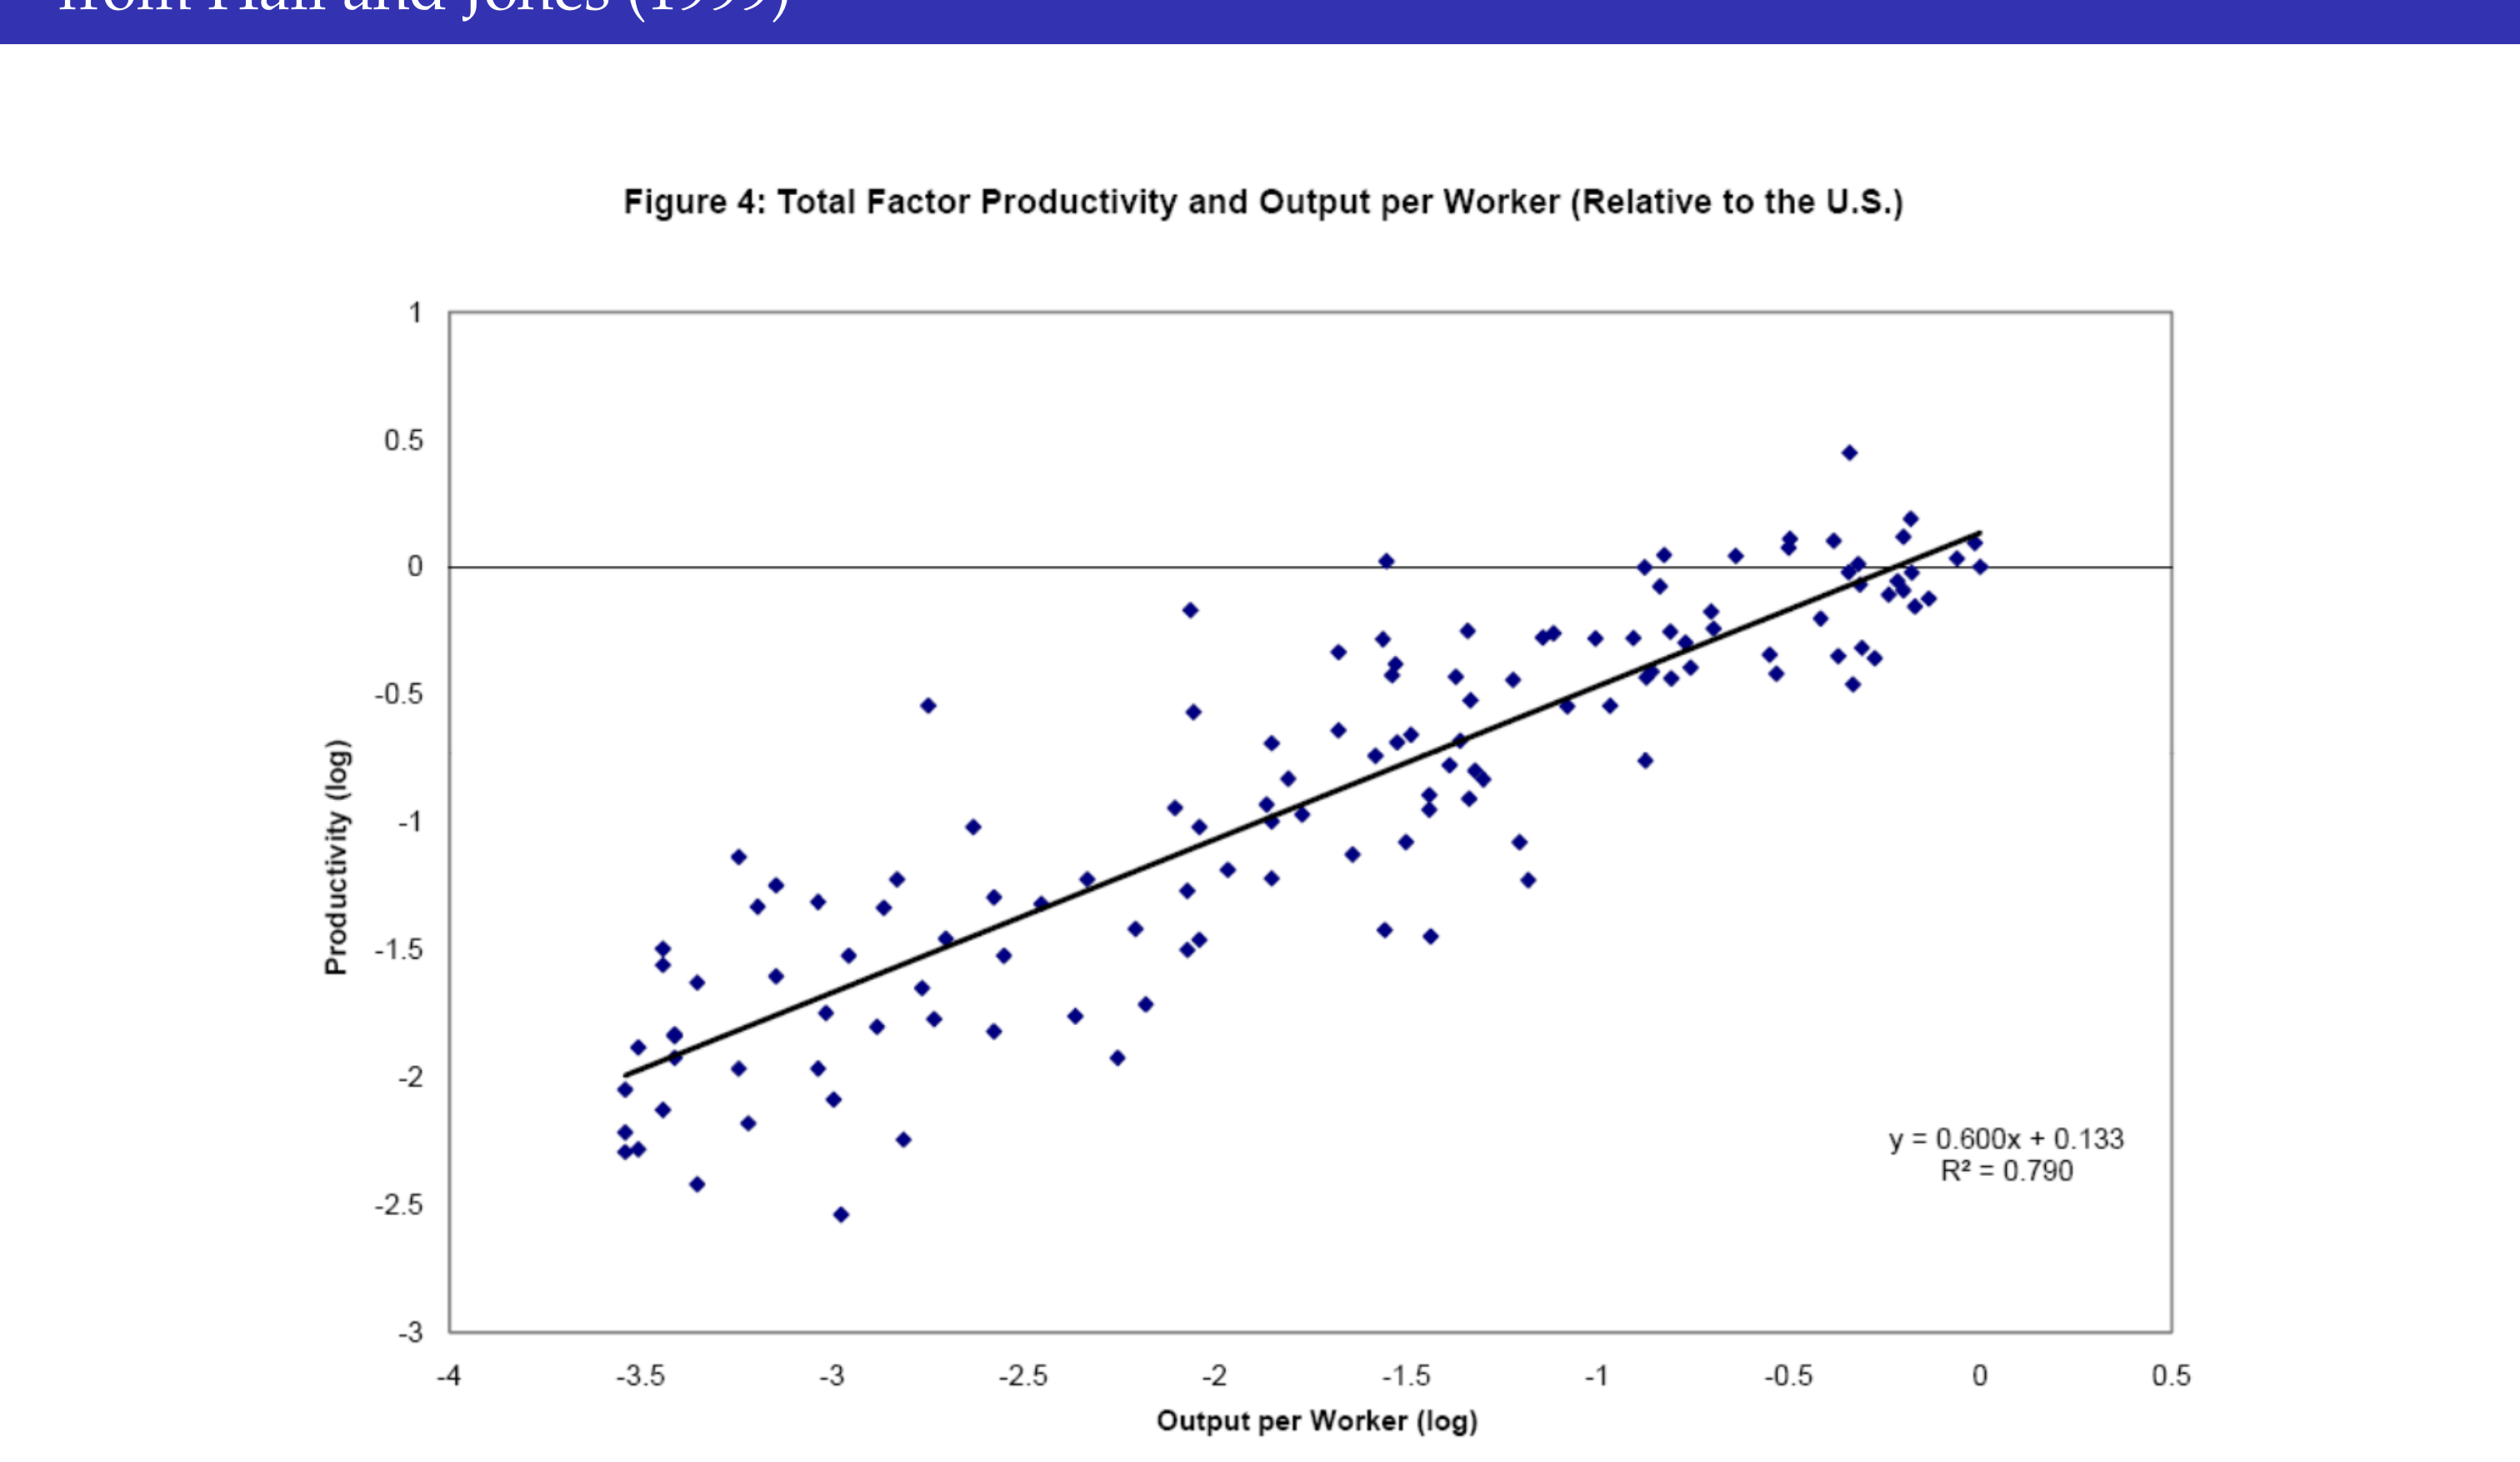
\includegraphics[width=0.95\textwidth]{topic4_p08_figure.png}
\end{frame}

\section{Baseline structure}

\begin{frame}{Structure housing endogenous growth models}
\small
\textbf{Households}
\begin{itemize}
    \item A constant large number of identical households (often normalized to $N=1$).
    \item Isoelastic utility over consumption:
    \[
    u(C)=\frac{C^{1-\sigma}-1}{1-\sigma}, \qquad \sigma>0.
    \]
    \item No valuation of leisure in the baseline version.
    \item Lifetime objective:
    \[
    \max \sum_{t=0}^{\infty} \beta^t u(C_t).
    \]
    \item Capital accumulation:
    \[
    K_{t+1}=(1-\delta)K_t+I_t.
    \]
\end{itemize}
\end{frame}

\begin{frame}{Structure housing endogenous growth models (continued)}
\small
\textbf{Final-goods producers}
\begin{itemize}
    \item Perfect competition in input and output markets.
    \item CRS production:
    \[
    Y = F(K,X),
    \]
    where $X$ is overall labor input or efficiency units of labor.
    \item Under CRS, we can write
    \[
    F(K,X)=Xf(k), \qquad k\equiv \frac{K}{X}.
    \]
    \item Competitive factor prices are:
    \[
    r+\delta = f'(k),
    \qquad
    w = f(k)-kf'(k).
    \]
\end{itemize}

\vspace{0.4em}
\textbf{Implication.} With perfect competition and CRS, total output is exhausted by factor payments, so profits are zero in equilibrium.
\end{frame}

\section{Why endogenous growth?}

\begin{frame}{Case 1: fixed labor-augmenting skills}
\small
Suppose
\[
Y_t = F(K_t, AN),
\]
where $A$ is constant.

\begin{itemize}
    \item If $A$ is fixed, then as $K_t$ rises, the capital--efficiency-labor ratio rises.
    \item Because $f'(k)$ is decreasing, the marginal product of capital falls.
    \item The Euler equation is
    \[
    u'(C_t)=\beta u'(C_{t+1})\big[f'(k_{t+1})+1-\delta\big].
    \]
    \item Sustained per-capita growth would require returns to remain high enough forever.
    \item But diminishing returns imply the economy converges to a steady state with \blue{no long-run per-capita growth}.
\end{itemize}

\vspace{0.3em}
So the standard neoclassical model needs \blue{exogenous technological progress} to explain persistent growth.
\end{frame}

\begin{frame}{Case 2: exogenously growing skills}
\small
Now let
\[
X_t=A_tN, \qquad A_t=\gamma_A A_{t-1}, \quad \gamma_A>1.
\]
Then
\[
Y_t = F(K_t,A_tN)=A_tN f\!\left(\frac{K_t}{A_tN}\right).
\]

\begin{itemize}
    \item If $K_t$ and $A_t$ grow at the same rate, then $k_t=K_t/(A_tN)$ stays constant.
    \item The marginal product of capital stays constant as well.
    \item Under isoelastic utility, the Euler equation implies
    \[
    \gamma_C^{\sigma} = \beta\big[f'(k)+1-\delta\big].
    \]
\end{itemize}

\vspace{0.4em}
This delivers balanced growth, but growth is still \blue{exogenous} because $A_t$ grows outside the model.
\end{frame}

\section{Endogenous growth mechanisms}

\begin{frame}{The AK model: the simplest endogenous growth model}
\small
Rebelo's AK model assumes
\[
Y = AK.
\]

\begin{itemize}
    \item The marginal product of capital is constant: \(MPK=A\).
    \item There are no diminishing returns to the accumulable factor.
    \item The Euler equation becomes
    \[
    \gamma_C^{\sigma}=\beta\big[A+1-\delta\big].
    \]
    \item If \(\beta[A+1-\delta]>1\), then consumption, capital, and output all grow forever.
\end{itemize}

\vspace{0.4em}
\textbf{Why is this important?}
\begin{itemize}
    \item It satisfies many Kaldor facts: constant return to capital, constant $K/Y$, and constant output growth.
    \item Policy can affect long-run growth directly.
\end{itemize}
\end{frame}

\begin{frame}{Policy matters in the AK model}
\small
Suppose output is taxed at rate $\tau$, so disposable output is
\[
Y^D=(1-\tau)AK.
\]
Then the Euler equation becomes
\[
\gamma_C^{\sigma}=\beta\big[(1-\tau)A+1-\delta\big].
\]

\begin{itemize}
    \item A higher output tax lowers the private return to accumulation.
    \item Therefore it lowers the economy's \blue{long-run growth rate}.
    \item This is a central distinction between exogenous-growth and endogenous-growth models:
    \begin{itemize}
        \item in exogenous-growth models, policy often affects levels but not long-run growth;
        \item in endogenous-growth models, policy can affect the \blue{growth rate itself}.
    \end{itemize}
\end{itemize}
\end{frame}

\begin{frame}{Learning by doing / external effects}
\small
Romer (1986) generates endogenous growth through a positive externality.

\begin{itemize}
    \item Let production be \(Y_t=F(K_t,X_t)\), with \(X_t=A_tN\).
    \item In equilibrium, knowledge evolves with aggregate capital, e.g.
    \[
    A_t = \frac{K_t}{N},
    \]
    but each firm takes $A_t$ as given.
    \item Privately, the firm sees CRS and chooses capital competitively.
    \item Socially, capital accumulation also raises knowledge, so there is an external return to investment.
\end{itemize}

\vspace{0.4em}
\textbf{Implications}
\begin{enumerate}
    \item constant growth in consumption and GDP is possible,
    \item policy can affect growth,
    \item the competitive equilibrium is generally \blue{not efficient} because firms ignore the knowledge spillover.
\end{enumerate}
\end{frame}

\begin{frame}{Takeaways}
\small
\begin{enumerate}
    \item Kaldor facts motivate balanced-growth analysis.
    \item Development accounting suggests that TFP is central for understanding income differences.
    \item With fixed technology, the neoclassical model does not generate sustained per-capita growth.
    \item Exogenous growth can be introduced through growing $A_t$, but that leaves the source of growth unexplained.
    \item Endogenous growth models explain long-run growth from economic forces inside the model:
    \begin{itemize}
        \item \blue{AK}: constant returns to accumulable capital,
        \item \blue{learning by doing}: external effects of accumulation,
        \item later models: R\&D, product variety, quality ladders, and human-capital accumulation.
    \end{itemize}
\end{enumerate}
\end{frame}

\end{document}
